\documentclass[a4paper,11pt]{exam}
\printanswers % pour imprimer les réponses (corrigé)
%\noprintanswers % Pour ne pas imprimer les réponses (énoncé)
\addpoints % Pour compter les points
% \noaddpoints % pour ne pas compter les points
%\qformat{\textbf{\thequestion ) } }
\qformat{\textbf{\thequestion )} (\thepoints) \\  } % Pour définir le style des questions (facultatif)
\usepackage{color} % définit une nouvelle couleur
\shadedsolutions % définit le style des réponses
% \framedsolutions % définit le style des réponses
\definecolor{SolutionColor}{rgb}{0.8,0.9,1} % bleu ciel
\renewcommand{\solutiontitle}{\noindent\textbf{Solution:}\par\noindent} % Définit le titre des solutions




\makeatletter

\def\maketitle{{\centering%
	\par{\huge\textbf{\@title}}%
	\par{\@date}%
	\par}}

\makeatother

\lhead{NOM Pr\'enom :}
\rhead{\textbf{Les r\'eponses doivent \^etre justifi\'ees}}
\cfoot{\thepage / \pageref{LastPage}}


%\usepackage{../../pas-math}
%\usepackage{../../moncours}


%\usepackage{pas-cours}
%-------------------------------------------------------------------------------
%          -Packages nécessaires pour écrire en Français et en UTF8-
%-------------------------------------------------------------------------------
\usepackage[utf8]{inputenc}
\usepackage[frenchb]{babel}
\usepackage[T1]{fontenc}
\usepackage{lmodern}
\usepackage{textcomp}



%-------------------------------------------------------------------------------

%-------------------------------------------------------------------------------
%                          -Outils de mise en forme-
%-------------------------------------------------------------------------------
\usepackage{hyperref}
\hypersetup{pdfstartview=XYZ}
%\usepackage{enumerate}
\usepackage{graphicx}
\usepackage{multicol}
\usepackage{tabularx}
\usepackage{multirow}


\usepackage{anysize} %%pour pouvoir mettre les marges qu'on veut
%\marginsize{2.5cm}{2.5cm}{2.5cm}{2.5cm}

\usepackage{indentfirst} %%pour que les premier paragraphes soient aussi indentés
\usepackage{verbatim}
\usepackage{enumitem}
\usepackage[usenames,dvipsnames,svgnames,table]{xcolor}

\usepackage{variations}

%-------------------------------------------------------------------------------


%-------------------------------------------------------------------------------
%                  -Nécessaires pour écrire des mathématiques-
%-------------------------------------------------------------------------------
\usepackage{amsfonts}
\usepackage{amssymb}
\usepackage{amsmath}
\usepackage{amsthm}
\usepackage{tikz}
\usepackage{xlop}
%-------------------------------------------------------------------------------



%-------------------------------------------------------------------------------


%-------------------------------------------------------------------------------
%                    - Mise en forme avancée
%-------------------------------------------------------------------------------

\usepackage{ifthen}
\usepackage{ifmtarg}


\newcommand{\ifTrue}[2]{\ifthenelse{\equal{#1}{true}}{#2}{$\qquad \qquad$}}

%-------------------------------------------------------------------------------

%-------------------------------------------------------------------------------
%                     -Mise en forme d'exercices-
%-------------------------------------------------------------------------------
%\newtheoremstyle{exostyle}
%{\topsep}% espace avant
%{\topsep}% espace apres
%{}% Police utilisee par le style de thm
%{}% Indentation (vide = aucune, \parindent = indentation paragraphe)
%{\bfseries}% Police du titre de thm
%{.}% Signe de ponctuation apres le titre du thm
%{ }% Espace apres le titre du thm (\newline = linebreak)
%{\thmname{#1}\thmnumber{ #2}\thmnote{. \normalfont{\textit{#3}}}}% composants du titre du thm : \thmname = nom du thm, \thmnumber = numéro du thm, \thmnote = sous-titre du thm

%\theoremstyle{exostyle}
%\newtheorem{exercice}{Exercice}
%
%\newenvironment{questions}{
%\begin{enumerate}[\hspace{12pt}\bfseries\itshape a.]}{\end{enumerate}
%} %mettre un 1 à la place du a si on veut des numéros au lieu de lettres pour les questions 
%-------------------------------------------------------------------------------

%-------------------------------------------------------------------------------
%                    - Mise en forme de tableaux -
%-------------------------------------------------------------------------------

\renewcommand{\arraystretch}{1.7}

\setlength{\tabcolsep}{1.2cm}

%-------------------------------------------------------------------------------



%-------------------------------------------------------------------------------
%                    - Racourcis d'écriture -
%-------------------------------------------------------------------------------

% Angles orientés (couples de vecteurs)
\newcommand{\aopp}[2]{(\vec{#1}, \vec{#2})} %Les deuc vecteurs sont positifs
\newcommand{\aopn}[2]{(\vec{#1}, -\vec{#2})} %Le second vecteur est négatif
\newcommand{\aonp}[2]{(-\vec{#1}, \vec{#2})} %Le premier vecteur est négatif
\newcommand{\aonn}[2]{(-\vec{#1}, -\vec{#2})} %Les deux vecteurs sont négatifs

%Ensembles mathématiques
\newcommand{\naturels}{\mathbb{N}} %Nombres naturels
\newcommand{\relatifs}{\mathbb{Z}} %Nombres relatifs
\newcommand{\rationnels}{\mathbb{Q}} %Nombres rationnels
\newcommand{\reels}{\mathbb{R}} %Nombres réels
\newcommand{\complexes}{\mathbb{C}} %Nombres complexes


%Intégration des parenthèses aux cosinus
\newcommand{\cosP}[1]{\cos\left(#1\right)}
\newcommand{\sinP}[1]{\sin\left(#1\right)}


%Probas stats
\newcommand{\stat}{statistique}
\newcommand{\stats}{statistiques}
%-------------------------------------------------------------------------------

%-------------------------------------------------------------------------------
%                    - Mise en page -
%-------------------------------------------------------------------------------

\newcommand{\twoCol}[1]{\begin{multicols}{2}#1\end{multicols}}


\setenumerate[1]{font=\bfseries,label=\textit{\alph*})}
\setenumerate[2]{font=\bfseries,label=\arabic*)}


%-------------------------------------------------------------------------------
%                    - Elements cours -
%-------------------------------------------------------------------------------




\usepackage{tabu}

%\usepackage{fullpage}
\author{\ }
\date{29 Novembre 2017}
\title{$1^{ère}$ $ST_2S$ : DS num\'ero 2}


\begin{document}
%	\usepackage{fancyhdr}
%	
%	\pagestyle{fancy}
%	\fancyhf{}
	%\rhead{Share\LaTeX}

	\maketitle





\section{Comparaison de deux suites (6 points)}

Les parents de Paul et Carine ont hérité d'une somme de \num{5000} € qu'ils offrent en deux parts égales à leurs enfants : chacun reçoit \num{2500} €.

Paul place la totalité de sa part sur un livret d'épargne aux taux de 2 \% par an à intérêts composés.

Carine place \num{1200} € sur un livret d'épargne à 4 \% à intérêts composés et garde le reste chez elle, dans sa tirelire.

On suppose que les deux enfants ne font plus désormais ni retrait ni versement.

\textit{Les résulats seront donnés à l'euro près}

\begin{questions}
	\question[2] 
	On note $S_n$ le capital de Paul au bout de $n$ années.
	\begin{parts}
		\part[1]  Calculer $S_1$, $S_2$, $S_3$.
			\begin{solution}
				\begin{itemize}
					\item $S_1 = S_0 \times \num{1.02}  = 2550 $ 
					\item $S_2 = 2601$ 
					\item $S_3 = 2653$
				\end{itemize}
				
			\end{solution}
		
		\part[1] $(S_n)$ est une suite géométrique, exprimer $S_n$ en fonction de $n$.
		\begin{solution}
			$S_n = 2500 \times \num{1.02}^{n}$
		\end{solution}
		
	\end{parts}
	
	\question[2] On note $T_n$, le capital total (livret et tirelire) de Carine au bout de $n$ années.
	\begin{parts}
		\part[1] Calculer $T_1$, $T_2$, $T_3$.
		\begin{itemize}
			\item $T_1 = 1200 \times \num{1.04} + 1300 = 1243 + 1300 = 2543 $ 
			\item $S_2 = 1243 \times \num{1.04} + 1300 = 1298 + 1300 = 2598 $ 
			\item $S_3 = 1298 \times \num{1.04} + 1300 = 1350 + 1300 = 2650 $ 
		\end{itemize}
		\part[1] Exprimer $T_n$ en fonction de $n$
		\begin{solution}
			$S_n = 1200 \times \num{1.04}^{n} + 1300$
		\end{solution}
	\end{parts}
	
	\question[1] Compléter le tableau suivant :
	
	\begin{center}
		
		\begin{tabular}{|@{$\quad $}c@{$\quad $}| @{$\qquad $}c@{$\qquad $} | @{$\qquad $}c@{$\qquad $} | @{$\qquad $}c@{$\qquad $} | @{$\qquad $}c@{$\qquad $} |@{$\qquad $}c@{$\qquad $} |@{$\qquad $}c@{$\qquad $} |@{$\qquad $}c@{$\qquad $}|@{$\qquad $}c@{$\qquad $}|}
			\hline
			$n$                           & 1 & 2 & 3 & 4 & 5 & 6 & 7 & 8 \\ \hline
			$S_n$ &   &   &   &   &   &   &   &   \\ \hline
			$T_n$ &   &   &   &   &   &   &   &   \\ \hline
		\end{tabular}
	\end{center}

	\begin{solution}
		\begin{small}
			
		\begin{center}
			
			\begin{tabular}{|@{$\quad $}c@{$\quad $}| @{\ }c@{\ } | @{\ }c@{\ } | @{\ }c@{\ } | @{\ }c@{\ } |@{\ }c@{\ } |@{\ }c@{\ } |@{\ }c@{\ }|@{\ }c@{\ }|}
				\hline
				$n$                           & 1 & 2 & 3 & 4 & 5 & 6 & 7 & 8 \\ \hline
				$S_n$ & 2550  & 2601  & 2653  & 2706  & 2760  & 2815  & 2872  & 2929  \\ \hline
				$T_n$ &  2548 &  2598 &  2650 &  2703 &  2759 &  2818 &  2879 &  2942 \\ \hline
			\end{tabular}
		\end{center}
		\end{small}
	\end{solution}
	
	\question[1] En déduire, en fonction du nombre d'années, qui de Paul ou de Carine, fait le meilleur placement.
	\begin{solution}
		Jusqu'à 6 ans, PAul à fait le meilleur placement, àrès 6 ans, c'est Carine.
	\end{solution}
	
\end{questions}

\section{Chiffre d'affaires (6 points)}

Le chiffre d'affaires d'un laboratoire pharmaceutique augmente tous les ans de \num{50000} €.
En 2007, le chiffre d'affaires était de \num{500000} €. On note $C_0 = \num{500000}$ et $C_n$ le chiffre d'affaires au cours de l'année $2007 + n$.

\begin{questions}
	\question[1] Exprimer pour tout entier $n$, $C_{n+1}$ en fonction de $C_n$.
	\begin{solution}
		$C_{n+1} = C_n + \num{50000}$
	\end{solution}

	\question
	\begin{parts}
		\part[1] En déduire que les nombres $C_0$, $C_1$, $C_2$, ... $C_n$ sont des termes successifs d'une suite arithmétique de premier terme $C_0$ dont on précisera la raison.
		\begin{solution}
			Tous les ans, le chiffre d'affaires augmente de \num{50000} €, donc pour passer d'un terme à l'autre an ajoute \num{50000}. J'en déduis qu'il s'agit d'une suite arithmétique de raison $r=\num{50000}$.
		\end{solution}
		
		\part[1] \`A quoi correspond $C_5$ ? Calculer $C_5$. 
		\begin{solution}
			$C_5$ représente le chiffre d'affaires du laboratoire en 2012 (2007 + 5 = 2012).
			
			On a $C_5 = \num{500000} + 5 \times \num{50000} = \num{750000}$ .
		\end{solution}
		
		\part[1] Calculer le chiffre d'affaires  prévisible pour 2013.
		\begin{solution}
			D'après la question $(a)$, je sais que $C_5$ correspond au chiffre d'affaires de l'année 2012. Donc pour 2013, il faut calculer $C_6$.
			
			On a : $C_6 = C_5 + \num{50000} =  \num{750000} + \num{50000} = \num{800000}$
		\end{solution}
	\end{parts}	
	
	\question[2] Déterminer en quelle année on peut prévoir un chiffre d'affaire de \num{1050000} €.
	\begin{solution}
		Je sais que $C_n = \num{500000} + n \times \num{50000}$.
		Je cherche la valeur de $n$ pour laquelle $C_n = \num{1050000}$ :
		
		\begin{eqnarray*}
			\num{1050000} &  = & \num{500000} + n \times \num{50000} \\
			\num{1050000} - \num{500000} & = & n \times \num{50000} \\
			\num{550000} & = & n \times \num{50000} \\
			\frac{\num{550000}}{\num{50000}} & = & n \\
			11 &=& n			
		\end{eqnarray*}
	
		Donc le chiffre d'affaires de \num{1050000} est atteint la 11$^e$ année, c'est à dire 2018.
	\end{solution}
	
\end{questions}

\section{La croissance du f\oe tus (8 points)}

Lors de la grossesse d'une femme, les médecins surveillent à l'aide de l'échographie, les médecins surveillent la croissance du f\oe tus durant les 39 semaines de grossesse.

Voici quelques indicateurs de cette surveillance :
\begin{itemize}
	\item Durant les premières semaines, on mesure la longueur du f\oe tus (longueur tête-fesses).
	\item Ensuite, lorsque le f\oe tus est trop grand pour être visualisé complètement sur l'écran et donc être mesuré, on s'intéresse à la dimension de sa tête. On mesure le diamètre bipariétal (l'écartement entre les deux os qui se trouvent de chaque coté de la face, au dessus des oreilles). Le graphique ci-dessous donne le diamètre bipariétal d'une f\oe tus entre les semaines 11 à 24.
	
	\begin{center}
		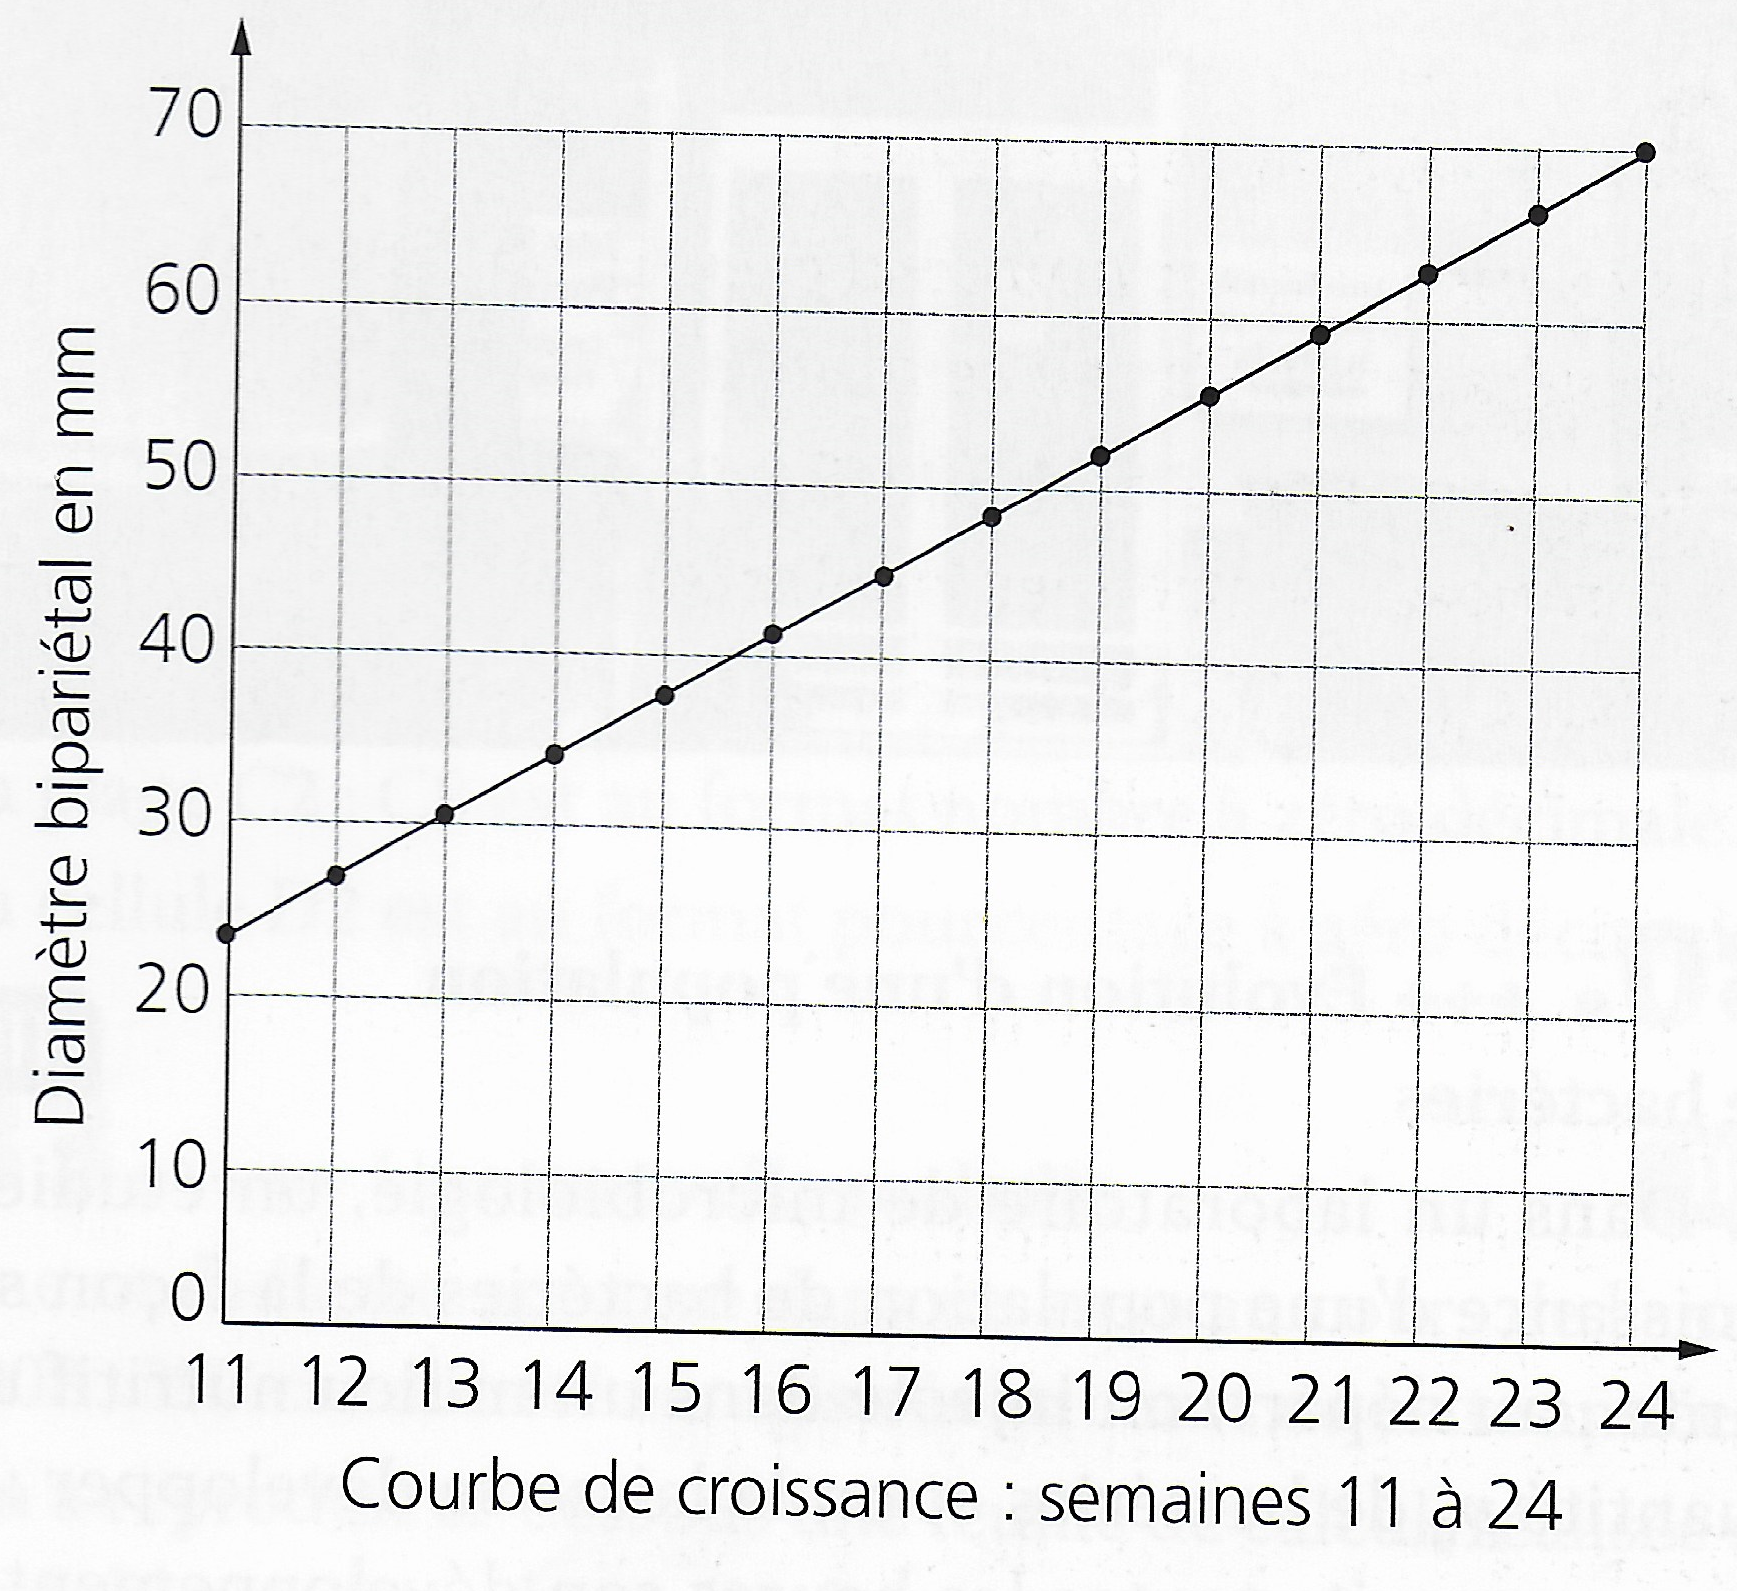
\includegraphics[scale=0.2]{graph_foetus}
	\end{center}

\end{itemize}


\begin{questions}
	\question[2] 
		\begin{parts}
			\part[1] Déterminer graphiquement le diamètre bipariétal au bout de 11 semaines.
			\begin{solution}
				Le diamètre bipariétal à 11 semaines est d'environ 25 mm.
			\end{solution}
			
			\part[1] On désigne par $u_{11}$, $u_{12}$, ..., $u_{24}$ les valeurs du diamètre bipariétal pour les semaines 11 à 24. Quelle semble être la nature de la suite formée par ces termes successifs ?
			\begin{solution}
				Les points représentant les termes de la suite sont alignés, donc la suite est arithmétique.
			\end{solution}
		\end{parts}
	
	\question[2]
		Dans cette question, on étudie la croissance du f\oe tus durant les semaines 4 à 10. Dans un tableur, on saisit les données concernant la taille du f\oe tus et on fait calculer le rapport entre deux valeurs consécutives.
		Les résultats sont donnés dans le tableau suivant :
		
		\begin{center}
			\includegraphics[scale=0.2]{tabl_foetus}
		\end{center}
		
		Pour simplifier, on retient \num{1.42} comme valeur approchée des résultats de la dernière colonne. Quelle est l'augmentation en pourcentage de la taille du f\oe tus en une semaine ?
		
		\begin{solution}
			\begin{equation*}
				\num{1.42} - 1 = \num{0.42}
			\end{equation*}
			
			Donc chaque semaine, la taille du f\oe tus augmente de 42 \%.
		\end{solution}
		
	\question[4]
		On considère la suite géométrique $(u_n)$ de raison \num{1.42} et telle que $u_0 = 7$. Le terme $u_n$ de rang $n$ représenterait la taille du f\oe tus en mm la semaine 4 + $n$.
		\begin{parts}
			\part[1] Que représenterait $u_{16}$ ?
				\begin{solution}
					$u_{16}$ représenterait la taille du f\oe tus en mm la semaine 20 (4 + 16).
				\end{solution}
			\part[1] Calculer une valeur approchée à l'unité de $u_{16}$.
				\begin{solution}
					\begin{eqnarray*}
						u_{16} & = & 7 \times \num{1.42}^{16} \\
						u_{16} & = & \num{1913}
					\end{eqnarray*}
				\end{solution}
			\part[2] Le modèle <<suite géométrique>> est-il pertinent au bout de 20 semaines ?
				\begin{solution}
					Si on suit ce modèle, à la vingtième semaine le f\oe tus mesurerait 1913 millimètres, soit presque 2 mètres. Ce n'est pas réaliste, donc le modèle n'est pas pertinent.
				\end{solution}
		\end{parts}
\end{questions}


	\label{LastPage}
	

\end{document}